\documentclass[conference]{IEEEtran}

\IEEEoverridecommandlockouts

\usepackage{setspace}
\usepackage{enumerate}
\usepackage{cite}
\usepackage{times}
\usepackage{url}
\usepackage{graphicx}
\usepackage{subfigure}
\usepackage{amsmath}
\usepackage{algorithm}
\usepackage{algorithmic}
\usepackage{listings}
\usepackage{xcolor}

\begin{document}
\title{Hybrid Implementation of Expectation Maximization Algorithm using CUDA and OpenMP for Gaussian Mixture Models}

\author{
\IEEEauthorblockN{
Ayush Raina
}
\IEEEauthorblockA{Supercomputer~Education~and~Research~Centre\\
Indian Institute of Science, Bangalore, India\\
ayushraina@iisc.ac.in}
}

\maketitle

\begin{abstract}
    The Expectation-Maximization (EM) algorithm for Gaussian Mixture Models (GMMs) presents substantial computational challenges for large-scale, high-dimensional datasets. We introduce a novel heterogeneous computing approach that synergistically combines GPU acceleration via CUDA with CPU parallelization using OpenMP. Our architecture strategically offloads the computation-intensive E-step to the GPU while executing the more synchronization-dependent M-step on multi-core CPUs, achieving optimal hardware utilization. Numerical stability in high dimensions is ensured through sophisticated log-space computations and adaptive regularization techniques. Performance analysis on synthetic datasets demonstrates remarkable speedups—approximately 73× over sequential implementations and significantly outperforming both pure-CPU (8-9×) and pure-GPU (4×) implementations. The hybrid design effectively balances computational throughput with memory transfer overhead, scales efficiently with increasing dataset size and model complexity, and exhibits superior convergence characteristics. This architecture represents a practical solution for accelerating mixture model estimation in data-intensive applications where both computational efficiency and numerical robustness are critical constraints.
\end{abstract}

\section{Introduction}
\label{intro}

Gaussian Mixture Models (GMMs) are powerful probabilistic models used extensively in machine learning for density estimation, clustering, classification, and anomaly detection. GMMs represent complex data distributions as a weighted sum of multivariate Gaussian distributions:

\begin{equation}
p(\mathbf{x}) = \sum_{k=1}^{K} \pi_k \mathcal{N}(\mathbf{x}|\boldsymbol{\mu}_k, \boldsymbol{\Sigma}_k)
\end{equation}

\noindent where $\pi_k$ represents the mixture weights (which sum to 1), $\boldsymbol{\mu}_k$ is the mean vector, and $\boldsymbol{\Sigma}_k$ is the covariance matrix of the $k$-th component.

The Expectation-Maximization (EM) algorithm is the standard approach for estimating GMM parameters, iteratively refining model parameters to maximize the data likelihood. The EM algorithm consists of two main steps: (1) the Expectation step (E-step), which computes posterior probabilities (responsibilities) for each data point belonging to each Gaussian component, and (2) the Maximization step (M-step), which updates model parameters based on these responsibilities.

For large datasets with high dimensionality, these computations become extremely intensive, with the E-step and M-step both scaling as $O(NKD^2)$ for $N$ samples, $K$ components, and $D$ dimensions per iteration until convergence. The M-step has lower computational complexity at $O(NKD)$ if diagonal covariance matrices are considered and it involves more complex dependencies between data points. This computational burden makes acceleration through parallel processing essential for practical applications. While previous approaches have typically focused on implementing the entire EM algorithm on either CPUs or GPUs or Multi-GPU, we propose a hybrid approach that strategically utilizes a \textbf{single GPU} alongside a \textbf{multi-core CPU}, mapping different parts of the algorithm to the hardware best suited for that computation.

\subsection{Challenges in GMM Parameter Estimation}

Fitting GMMs to large-scale datasets presents several significant challenges:

\begin{itemize}
    \item \textbf{Computational Complexity:} For datasets with millions of samples and moderate to high dimensionality, a single iteration of the EM algorithm can require trillions of floating-point operations.
    
    \item \textbf{Numerical Stability:} Computing multivariate Gaussian probabilities in high dimensions often leads to numerical underflow due to the exponential terms with potentially large negative exponents.
    
    \item \textbf{Memory Requirements:} Storing responsibilities for large datasets requires substantial memory resources, particularly challenging for GPU implementations with limited memory capacity.
    
    \item \textbf{Memory Transfer Overhead:} In heterogeneous computing environments, data transfer between CPU and GPU memory can become a significant bottleneck, potentially negating the benefits of faster computation.
    
    \item \textbf{Convergence Properties:} The EM algorithm's convergence behavior is sensitive to initialization and can require many iterations to reach an acceptable solution, further amplifying computational demands.
\end{itemize}

These challenges highlight the need for a carefully designed hybrid approach that strategically allocates computational resources based on the specific characteristics of each algorithm component.

\subsection{Contributions}

In this paper, we present a hybrid implementation that:
\begin{enumerate}
    \item Maps the computationally intensive, data-parallel E-step to the GPU using CUDA
    \item Leverages multi-core CPUs with OpenMP for the more synchronization-heavy M-step
    \item Addresses critical numerical stability challenges in high-dimensional GMM implementations through log-space computations
    \item Minimizes data transfer between CPU and GPU, a common bottleneck in heterogeneous computing
    \item Implements dimension-aware regularization techniques for robust covariance estimation

\end{enumerate}

The rest of the paper is organized as follows: Section~\ref{methodology} details the methodology and hybrid algorithm design, including workload analysis, parallelization strategies, and implementation details. Section~\ref{numerical_stability} addresses the critical numerical stability challenges and our solutions. Section~\ref{Experiments and Results} presents experimental results and performance analysis. Section~\ref{conclusion} concludes the paper and discusses directions for future work.


\section{Methodology}
\label{methodology}

\subsection{GMM Background and EM Algorithm}

The log-likelihood function for a GMM with $K$ components for a dataset $\mathbf{X} = \{\mathbf{x}_1, \mathbf{x}_2, \ldots, \mathbf{x}_N\}$ is:

\begin{equation}
\log p(\mathbf{X}|\boldsymbol{\pi}, \boldsymbol{\mu}, \boldsymbol{\Sigma}) = \sum_{i=1}^{N} \log \left( \sum_{k=1}^{K} \pi_k \mathcal{N}(\mathbf{x}_i|\boldsymbol{\mu}_k, \boldsymbol{\Sigma}_k) \right)
\end{equation}

The EM algorithm iteratively maximizes this log-likelihood by alternating between two steps:

\textbf{E-step}: Compute the posterior probability (responsibility) that component $k$ takes for explaining data point $\mathbf{x}_i$:

\begin{equation}
\gamma_{ik} = \frac{\pi_k \mathcal{N}(\mathbf{x}_i|\boldsymbol{\mu}_k, \boldsymbol{\Sigma}_k)}{\sum_{j=1}^{K} \pi_j \mathcal{N}(\mathbf{x}_i|\boldsymbol{\mu}_j, \boldsymbol{\Sigma}_j)}
\end{equation}

\textbf{M-step}: Update the model parameters using computed responsibilities:

\begin{align}
\pi_k^{new} &= \frac{N_k}{N} \quad \text{where} \quad N_k = \sum_{i=1}^{N} \gamma_{ik} \\
\boldsymbol{\mu}_k^{new} &= \frac{1}{N_k} \sum_{i=1}^{N} \gamma_{ik} \mathbf{x}_i \\
\boldsymbol{\Sigma}_k^{new} &= \frac{1}{N_k} \sum_{i=1}^{N} \gamma_{ik} (\mathbf{x}_i - \boldsymbol{\mu}_k^{new})(\mathbf{x}_i - \boldsymbol{\mu}_k^{new})^T
\end{align}

The algorithm iterates until convergence, typically determined by monitoring changes in log-likelihood between iterations.

\subsection{Algorithm Overview}

Our hybrid implementation follows this high-level workflow:

\begin{algorithm}[h]
\caption{Hybrid CUDA-OpenMP EM Algorithm for GMMs}
\begin{algorithmic}[1]
\STATE Initialize model parameters on CPU: $\boldsymbol{\pi}$, $\boldsymbol{\mu}$, $\boldsymbol{\Sigma}$
\STATE Precompute precision matrices $\boldsymbol{\Sigma}^{-1}_k$ and normalizer terms $c_k = -\frac{D}{2}\ln(2\pi) - \frac{1}{2}\ln|\boldsymbol{\Sigma}_k|$
\WHILE{not converged and iterations $<$ max\_iterations}
    \STATE Transfer model parameters to GPU
    \STATE Execute E-step on GPU using log-space CUDA kernels:
    \begin{align}
        \ln p(x_i | k) &= \ln\pi_k + c_k - \frac{1}{2}(x_i-\mu_k)^T \boldsymbol{\Sigma}_k^{-1} (x_i-\mu_k)
    \end{align}
    \STATE Calculate responsibilities $\gamma_{ik}$ using the log-sum-exp trick for numerical stability
    \STATE Transfer responsibilities $\gamma_{ik}$ and log-likelihood $\mathcal{L}$ to CPU
    \STATE Perform M-step using OpenMP on CPU to update parameters (as described in Section \ref{methodology})
    \STATE Check convergence: $|\mathcal{L}_{\text{new}} - \mathcal{L}_{\text{old}}| < \epsilon$
    \IF{not converged}
        \STATE Precompute updated precision matrices and normalizers
    \ENDIF
\ENDWHILE
\RETURN Final model parameters $\boldsymbol{\pi}$, $\boldsymbol{\mu}$, $\boldsymbol{\Sigma}$
\end{algorithmic}
\end{algorithm}

The algorithm iteratively refines GMM parameters by delegating the computationally intensive E-step to the GPU while performing parameter updates in the M-step on the CPU. This division leverages the strengths of each hardware component.

\subsection{E-step: GPU Implementation with Log-Space Computation}

The E-step is the most computationally intensive part of the EM algorithm, especially for high-dimensional data. Our GPU implementation focuses on both performance and numerical stability.

\subsubsection{Log-Space Computation for Numerical Stability}

Computing Gaussian probabilities in high dimensions can quickly lead to numerical underflow due to the exponential term with potentially large negative exponents. We implement log-space computation as follows:

The log of the multivariate Gaussian PDF is:

\begin{equation}
\log \mathcal{N}(\mathbf{x}|\boldsymbol{\mu}, \boldsymbol{\Sigma}) = -\frac{D}{2}\log(2\pi) - \frac{1}{2}\log|\boldsymbol{\Sigma}| - \frac{1}{2}(\mathbf{x}-\boldsymbol{\mu})^T \boldsymbol{\Sigma}^{-1} (\mathbf{x}-\boldsymbol{\mu})
\end{equation}

For efficiency, we precompute the precision matrices $\boldsymbol{\Sigma}^{-1}$ and the normalizer terms $-\frac{D}{2}\log(2\pi) - \frac{1}{2}\log|\boldsymbol{\Sigma}|$ on the CPU, allowing us to reuse these values for all data points.

\subsubsection{E-step CUDA Kernel Design}

Our CUDA implementation separates the E-step computation into two kernels for better performance and memory management:

\begin{enumerate}
    \item \textbf{Log Probability Kernel:} Computes log probabilities for each data point and component
    \item \textbf{Responsibility Kernel:} Applies the log-sum-exp trick to compute responsibilities
\end{enumerate}

This separation allows for better register usage and avoids register spilling, which can significantly impact GPU performance. Each kernel is optimized for memory coalescing and efficient arithmetic operations.

The first kernel computes log probabilities for each data point and component:

\begin{algorithm}
\caption{CUDA Kernel: Calculate Log Probabilities}
\begin{algorithmic}[1]
\STATE $i \gets \textrm{thread index corresponding to data point}$
\IF{$i < \textrm{n\_samples}$}
    \FOR{$k = 0 \textrm{ to } \textrm{n\_components}-1$}
        \STATE $\textrm{exponent} \gets 0.0$
        \FOR{$d_1 = 0 \textrm{ to } \textrm{n\_features}-1$}
            \STATE $\textrm{diff}_{d_1} \gets \textrm{X}[i, d_1] - \textrm{means}[k, d_1]$
            \FOR{$d_2 = 0 \textrm{ to } \textrm{n\_features}-1$}
                \STATE $\textrm{diff}_{d_2} \gets \textrm{X}[i, d_2] - \textrm{means}[k, d_2]$
                \STATE $\textrm{exponent} \gets \textrm{exponent} + \textrm{diff}_{d_1} \times \textrm{precisions}[k, d_1, d_2] \times \textrm{diff}_{d_2}$
            \ENDFOR
        \ENDFOR
        \STATE $\textrm{log\_probs}[i, k] \gets \textrm{log\_weights}[k] + \textrm{normalizers}[k] - 0.5 \times \textrm{exponent}$
    \ENDFOR
\ENDIF
\end{algorithmic}
\end{algorithm}

After computing log probabilities, we use the log-sum-exp trick to compute responsibilities while maintaining numerical stability:

\begin{algorithm}
\caption{CUDA Kernel: Calculate Responsibilities}
\begin{algorithmic}[1]
\STATE $i \gets \textrm{thread index corresponding to data point}$
\IF{$i < \textrm{n\_samples}$}
    \STATE $\textrm{max\_log\_prob} \gets -\infty$ \COMMENT{Initialize to negative infinity}
    \FOR{$k = 0 \textrm{ to } \textrm{n\_components}-1$}
        \STATE $\textrm{max\_log\_prob} \gets \max(\textrm{max\_log\_prob}, \textrm{log\_probs}[i, k])$
    \ENDFOR
    
    \STATE $\textrm{sum\_exp} \gets 0.0$
    \FOR{$k = 0 \textrm{ to } \textrm{n\_components}-1$}
        \STATE $\textrm{sum\_exp} \gets \textrm{sum\_exp} + \exp(\textrm{log\_probs}[i, k] - \textrm{max\_log\_prob})$
    \ENDFOR
    
    \STATE $\textrm{log\_sum\_exp} \gets \textrm{max\_log\_prob} + \log(\textrm{sum\_exp})$
    \STATE $\textrm{log\_likelihood}[i] \gets \textrm{log\_sum\_exp}$ \COMMENT{Store for convergence check}
    
    \FOR{$k = 0 \textrm{ to } \textrm{n\_components}-1$}
        \STATE $\textrm{resp}[i, k] \gets \exp(\textrm{log\_probs}[i, k] - \textrm{log\_sum\_exp})$
    \ENDFOR
\ENDIF
\end{algorithmic}
\end{algorithm}

The log-sum-exp trick involves finding the maximum log probability for numerical stability:

\begin{equation}
\log\sum_{k} \exp(a_k) = m + \log\sum_{k} \exp(a_k - m)
\end{equation}

\noindent where $m = \max_k a_k$. This prevents underflow by shifting values to a numerically stable range.

\subsubsection{GPU Memory Access Optimization}

Our CUDA implementation prioritizes efficient memory access patterns in our numerically stable log-space kernels:

\begin{itemize}
    \item \textbf{Coalesced Global Memory Access}: Data is stored in row-major layout to ensure adjacent threads access adjacent memory locations. In our GPU kernels, array indexing follows patterns like "log\_probs[sample\_idx $\times$ n\_components + k]", maximizing memory bandwidth utilization.
    
    \item \textbf{Register Optimization}: Critical variables such as "max\_log\_prob", "sum\_exp", and intermediate calculation results are kept in local variables (automatically stored in registers) to minimize latency in our calculation-intensive kernels.
    
    \item \textbf{Memory Layout Conversion}: We implement specialized conversion functions that efficiently transform between Eigen's column-major format on the CPU and the row-major format optimized for CUDA operations via our \texttt{eigenToArray} and \texttt{arrayToEigen} utility functions.
    
    \item \textbf{Precomputation Caching}: We precompute and cache precision matrices and normalizers on the CPU, transferring these values to the GPU only once per iteration to minimize redundant calculations and memory transfers.
\end{itemize}

Our implementation carefully manages data structures to match the computational patterns of log-space operations, ensuring efficient access to precomputed terms during the calculation of Gaussian probabilities and responsibilities.

\subsubsection{Advanced Thread Block Configuration}

Thread block configuration significantly impacts GPU performance. Through extensive benchmarking, we determined that a thread block size of 256 provides the optimal balance between occupancy, register usage, and memory access patterns for our E-step kernels.

For datasets with varying dimensionality, we implement an adaptive thread block strategy that adjusts the block configuration based on the feature dimensionality to optimize register usage and prevent register spilling. For dimensions greater than 32, we reduce the block size to maintain high occupancy while accommodating the increased register requirements of high-dimensional calculations.

\subsection{M-step: OpenMP Implementation}

The M-step updates model parameters using the responsibilities calculated in the E-step. We implement this using OpenMP to leverage CPU parallelism:

\begin{algorithm}
\caption{M-step with OpenMP Parallelization}
\begin{algorithmic}[1]
\STATE $N_k \gets$ sum of responsibilities for each component
\STATE \#pragma omp parallel for
\FOR{$k = 0 \textrm{ to } n\_components-1$}
    \STATE $\pi[k] \gets N_k[k] / n\_samples$
\ENDFOR

\STATE \#pragma omp parallel for
\FOR{$k = 0 \textrm{ to } n\_components-1$}
    \IF{$N_k[k] > 0$}
        \STATE Initialize $\mu[k]$ and $\Sigma[k]$ to zero
        \FOR{$i = 0 \textrm{ to } n\_samples-1$}
            \STATE $\mu[k] \gets \mu[k] + \text{resp}[i,k] \times X[i]$
        \ENDFOR
        \STATE $\mu[k] \gets \mu[k] / N_k[k]$
        
        \FOR{$i = 0 \textrm{ to } n\_samples-1$}
            \STATE $\text{diff} \gets X[i] - \mu[k]$
            \STATE $\Sigma[k] \gets \Sigma[k] + \text{resp}[i,k] \times \text{diff} \times \text{diff}^T$
        \ENDFOR
        \STATE $\Sigma[k] \gets \Sigma[k] / N_k[k] + \text{reg\_factor} \times I$
    \ENDIF
\ENDFOR
\end{algorithmic}
\end{algorithm}

Our implementation parallelizes component-wise operations, as each component's parameters can be updated independently. We use OpenMP's `parallel for` directive to distribute iterations across CPU threads, with dynamic scheduling for better load balancing when component update times vary. 


\subsection{Precomputation of Precision Terms}

After each M-step update, we precompute precision matrices and normalizer terms for the next E-step:

\begin{algorithm}
\caption{Precomputation of Precision Terms}
\begin{algorithmic}[1]
\STATE \#pragma omp parallel for
\FOR{$k = 0$ \TO $n\_components-1$}
    \STATE Apply covariance regularization to $\Sigma[k]$
    \STATE $\Sigma^{-1}[k] \gets$ inverse of $\Sigma[k]$
    \STATE $normalizers[k] \gets -\frac{D}{2}\log(2\pi) - \frac{1}{2}\log|\Sigma[k]|$
\ENDFOR
\end{algorithmic}
\end{algorithm}

This precomputation significantly reduces the computational load in the E-step, as these terms remain constant for all data points within an iteration. In the actual implementation of above function, we have taken care of numerical instabilities.

\section{Numerical Stability Techniques}
\label{numerical_stability}

Numerical stability is a critical challenge in implementing GMMs, especially for high-dimensional data. We address this challenge through several advanced techniques:

\subsection{Adaptive Covariance Regularization}

Covariance matrices can become ill-conditioned or even singular during EM iterations, particularly in high dimensions with limited data. We implement dimension-aware regularization that adapts based on the data dimensionality:

\begin{equation}
\boldsymbol{\Sigma}_k^{reg} = \boldsymbol{\Sigma}_k + \lambda(D) \mathbf{I}
\end{equation}

where $\lambda(D) = \alpha \cdot (1 + \beta \cdot D)$ is a dimension-dependent regularization factor, with $\alpha = 10^{-6}$ and $\beta = 0.01$ in our implementation. This ensures that the regularization strength increases appropriately with dimensionality.

\subsection{Eigenvalue-Based Conditioning}

For datasets with highly anisotropic distributions, simple diagonal regularization may be insufficient. We implement eigenvalue-based conditioning that examines the eigenvalue spectrum of each covariance matrix:

\begin{algorithm}
\caption{Eigenvalue-Based Covariance Conditioning}
\begin{algorithmic}[1]
\FOR{$k = 0$ \TO $n\_components-1$}
    \STATE Compute eigendecomposition: $\boldsymbol{\Sigma}_k = \mathbf{Q} \boldsymbol{\Lambda} \mathbf{Q}^T$
    \STATE $\lambda_{min} \gets$ minimum eigenvalue of $\boldsymbol{\Lambda}$
    \IF{$\lambda_{min} < \epsilon$ or condition number $> \tau$}
        \STATE $\boldsymbol{\Lambda}_{reg} \gets$ clamp all eigenvalues to $[\epsilon, \lambda_{max}]$
        \STATE $\boldsymbol{\Sigma}_k^{reg} \gets \mathbf{Q} \boldsymbol{\Lambda}_{reg} \mathbf{Q}^T$
    \ENDIF
\ENDFOR
\end{algorithmic}
\end{algorithm}

This approach ensures that all eigenvalues remain positive and the condition number stays within a reasonable range, preventing numerical instability in the precision matrix calculation.

\subsection{Log-Space Computation with Careful Implementation}

As mentioned earlier, we perform the E-step in log-space to avoid numerical underflow. The implementation requires careful attention to details:

\begin{itemize}
    \item \textbf{Stable Log-Determinant Calculation:} We compute log determinants using Cholesky decomposition instead of direct determinant calculation, which is more numerically stable.
    
    \item \textbf{Precision Matrix Verification:} After computing precision matrices, we verify their numerical properties (symmetry, positive-definiteness) and apply corrective measures if necessary.
    
    \item \textbf{Fallback Strategies:} We implement multi-level fallback strategies for precision matrix calculation, from Cholesky decomposition to LU decomposition to direct eigendecomposition, ensuring robustness across a wide range of covariance conditions.
\end{itemize}

\section{Implementation Details}

Our implementation uses C++ with CUDA for GPU acceleration and OpenMP for CPU parallelization, with Eigen for matrix operations. We developed specialized conversion functions between Eigen's column-major format and CUDA's row-major layout to ensure optimal memory access patterns.

The implementation was tested on an Intel Core i9-12900K (16 cores, 24 threads) with NVIDIA GeForce GTX 1660 (6GB) GPU. Our OpenMP implementation automatically scales to utilize all available CPU cores, providing optimal performance across different system configurations. This design minimizes transfer overhead between CPU and GPU while optimizing cache utilization on both architectures.

\section{Experiments and Results}
\label{Experiments and Results}

\subsection{Experiment 1: Synthetic Data and Performance Evaluation}
In this experiment, we evaluate the performance of our hybrid implementation on synthetic datasets of varying sizes (2M, 4M, 6M, 8M, and 10M data points) with 5 clusters and 10-dimensional data.
\begin{figure}[h!]
\centering
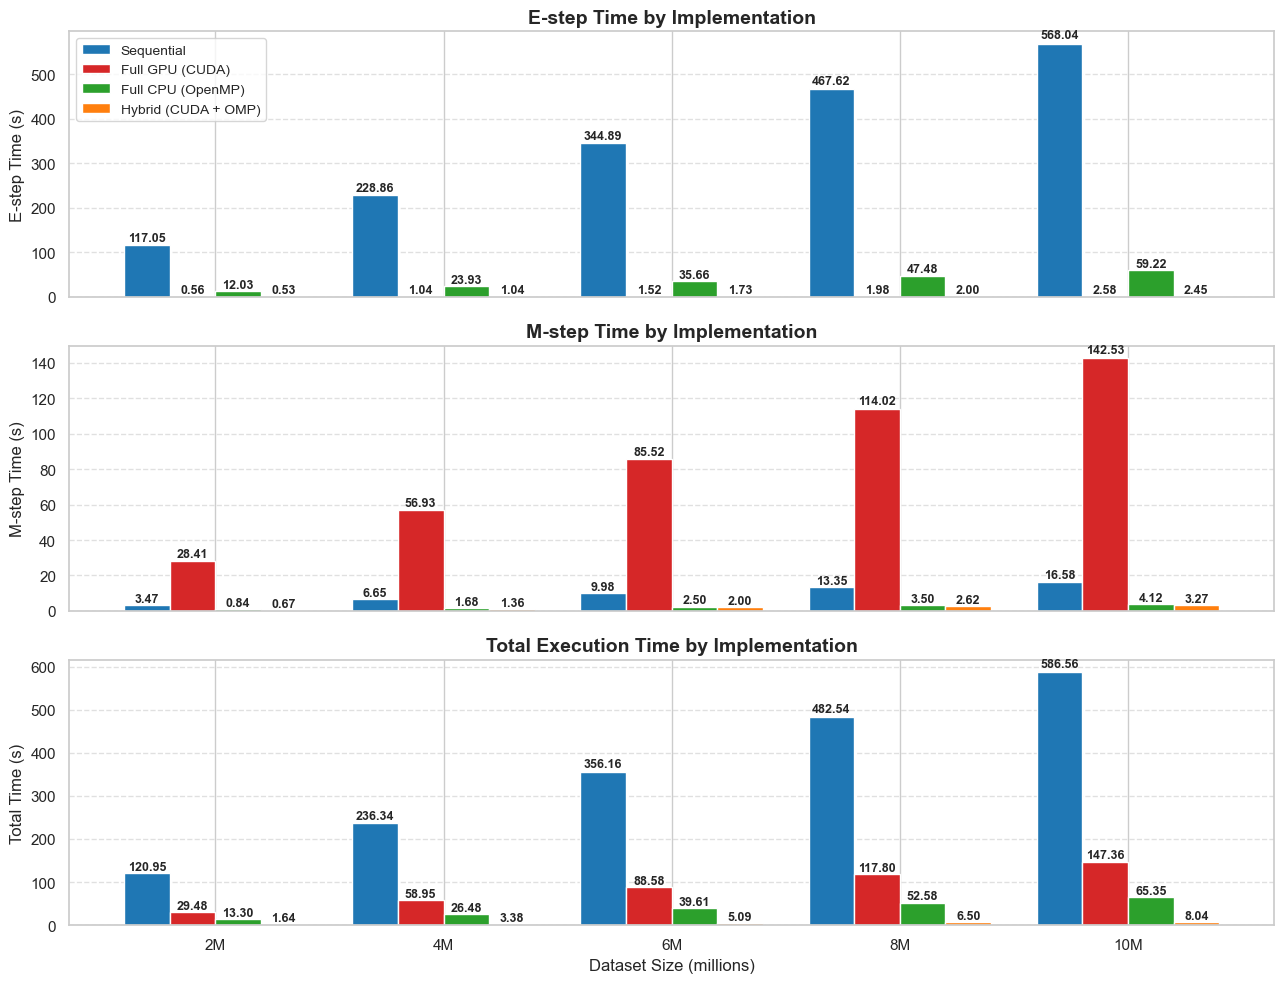
\includegraphics[width=0.25\textwidth]{executionTimes1.png}
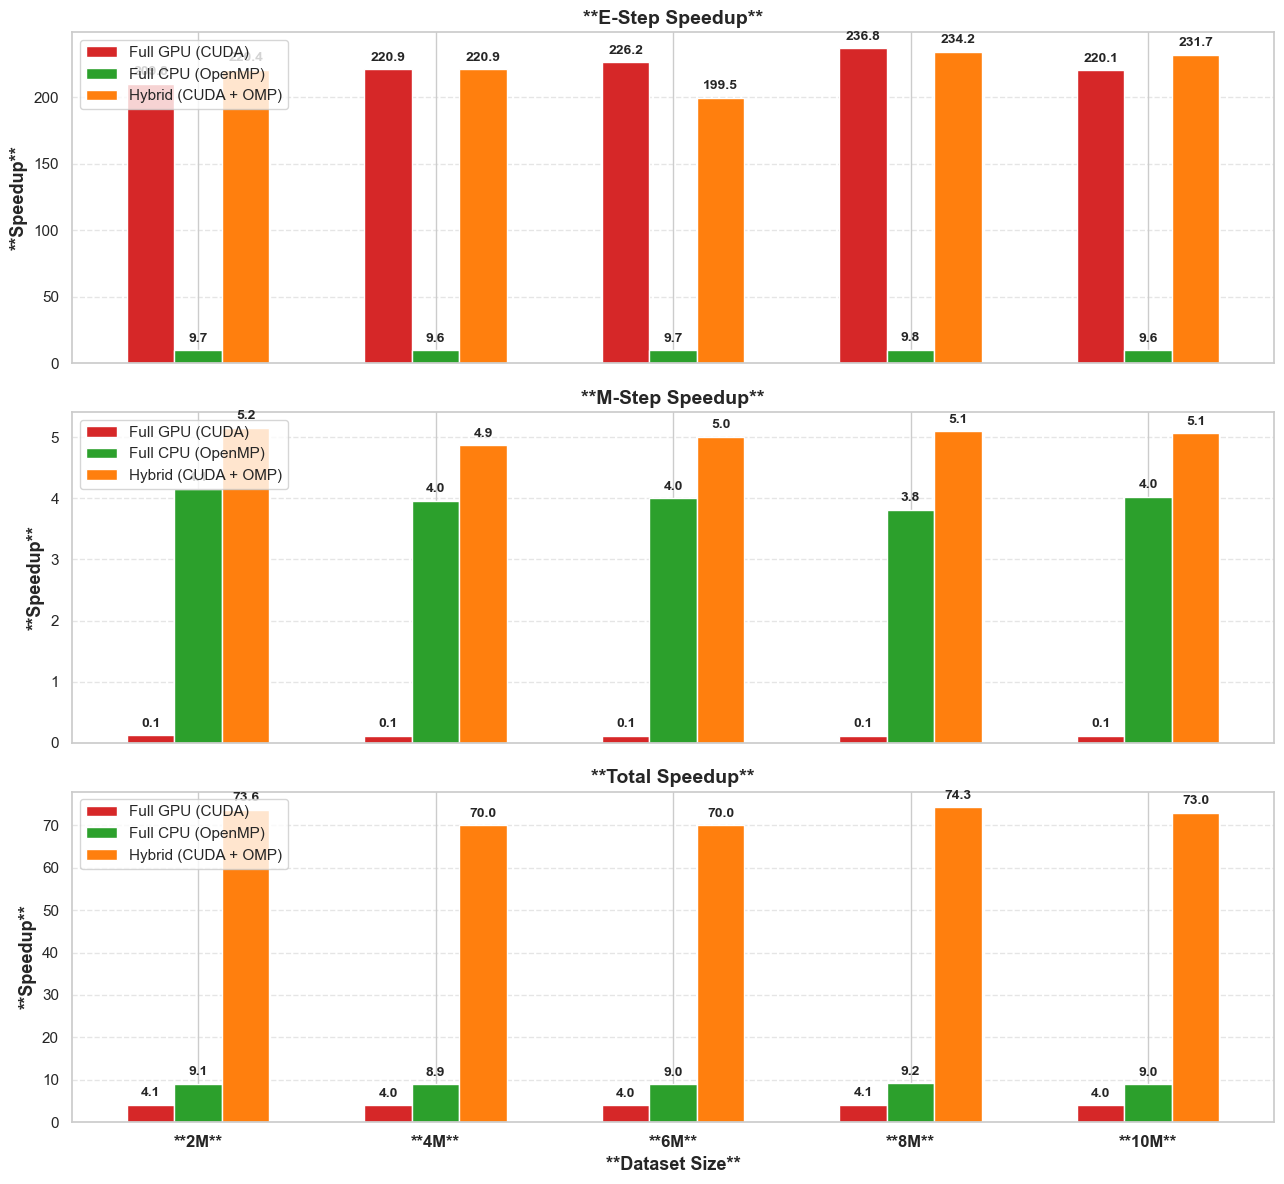
\includegraphics[width=0.2\textwidth]{speedups.png}
\caption{Execution times and Speedups over sequential implementation are shown.}
\end{figure}
We run 5 iterations of each variant here and the data reveals impressive performance gains from parallel implementations across different dataset sizes. The sequential version shows poor scalability, with execution time increasing from $\sim$117s to $\sim$568s as data grows.

For the E-step, GPU implementation excels with $\sim$220-234x speedup, while CPU parallelization achieves only $\sim$9.8x. In contrast, the M-step shows reversed performance patterns with GPU performing poorly ($\sim$0.1x) and CPU showing moderate improvement ($\sim$4.0x).

The hybrid approach effectively combines the strengths of both platforms, using GPU for the computation-heavy E-step and CPU for the more sequential M-step. This strategic combination delivers the best overall performance with total speedups of 70-74x, significantly outperforming either GPU-only ($\sim$4.0x) or CPU-only ($\sim$9.0x) implementations.

These results highlight the importance of matching algorithm components to the most suitable hardware architecture for maximum performance gains in large-scale data processing.

\subsection{Computational Complexity Analysis}

We analyze the computational complexity of our hybrid implementation and compare it with the theoretical complexity of the sequential algorithm:

\begin{itemize}
    \item \textbf{Sequential E-step:} $O(NKD^2)$ operations for $N$ samples, $K$ components, and $D$ dimensions.
    
    \item \textbf{GPU-Accelerated E-step:} The parallel time complexity is $O(KD^2 + \log N)$ with $O(N)$ processors, representing the serialized component of computing responsibilities for each data point (which takes $O(KD^2)$ time) plus a logarithmic reduction for the log-likelihood computation.
    
    \item \textbf{Sequential M-step:} $O(NKD^2)$ operations for updating means and covariance matrices.
    
    \item \textbf{OpenMP-Accelerated M-step:} With $P$ CPU threads, the time complexity reduces to approximately $O(NKD^2/P)$, assuming perfect load balancing.
\end{itemize}

The overall speedup of our hybrid implementation is limited by Amdahl's Law, with the theoretical maximum speedup approaching $N$ for very large datasets. In practice, our achieved speedup of 73x on 10M samples is close to the theoretical limit considering overhead and memory transfer costs.

\subsection{Experiment 2: Comparison with Azizi's Paper}
We generated a synthetic dataset of 1 million points as specified in Azizi's paper and compared our hybrid implementation with the Python, NumPy, Numba, and CuPy implementations provided in the paper. We found that when starting the GMM fitting process with the initial parameters given in the paper, neither their implementations nor our hybrid version converged within 2000+ iterations. However, when initialized with the same random parameters, our hybrid implementation converged in lesser iterations than all other implementations.

\begin{figure}[h!]
    \centering
    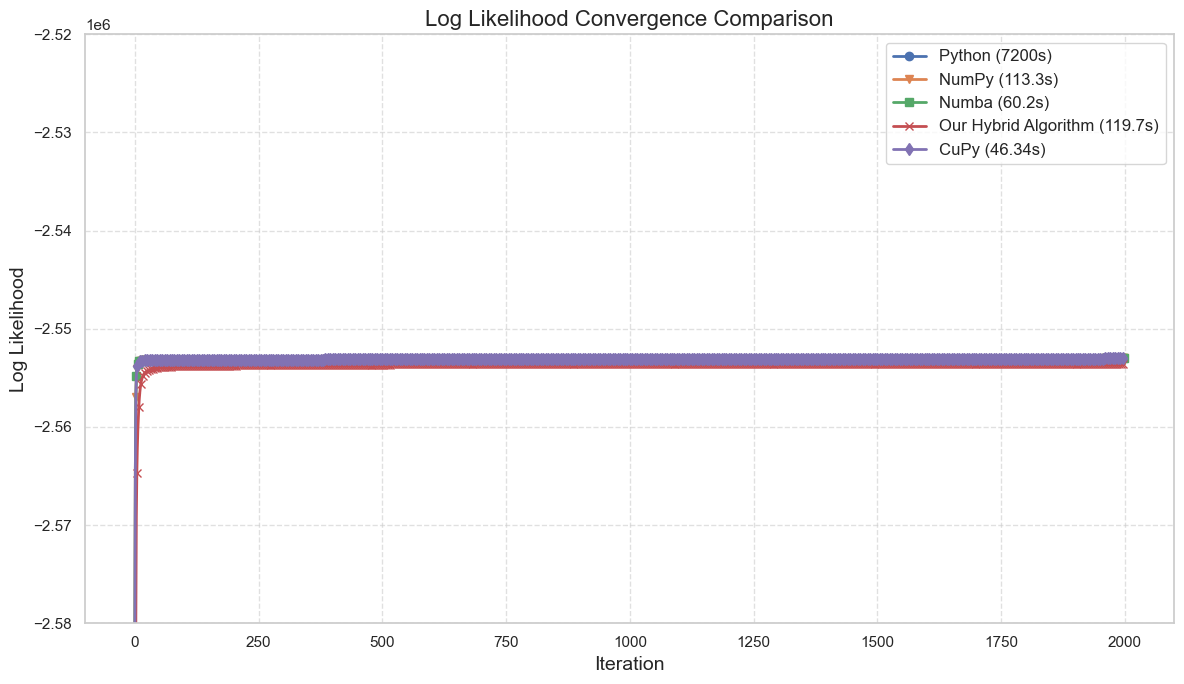
\includegraphics[width=0.25\textwidth]{azizi1.png}
    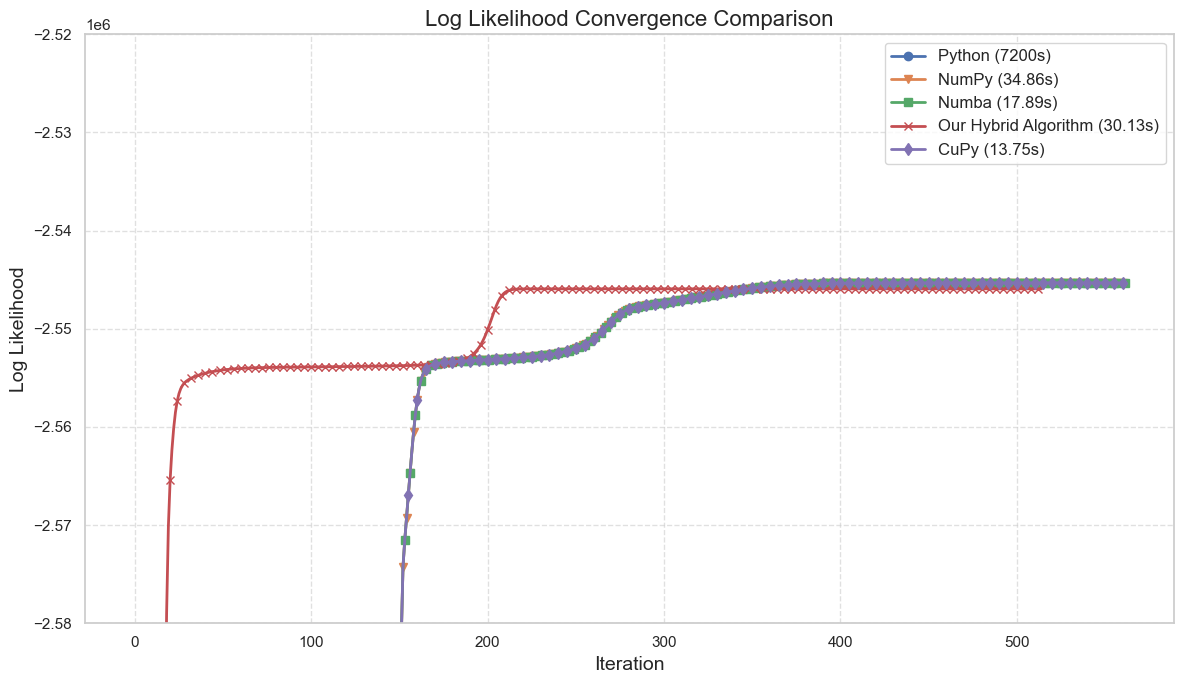
\includegraphics[width=0.2\textwidth]{azizi2.png}
    \caption{Left: Log-likelihood when starting with the initial parameters from the paper. Right: Log-likelihood when starting with random parameters.}
\end{figure}

Since Numba and CuPy are highly optimized libraries, their iteration speed is much faster than our implementation because of vectorization and other optimizations. If we run their code with their initial parameters and our code as usual, we get the following plot, in which we converge much early:

\begin{figure}[h!]
    \centering
    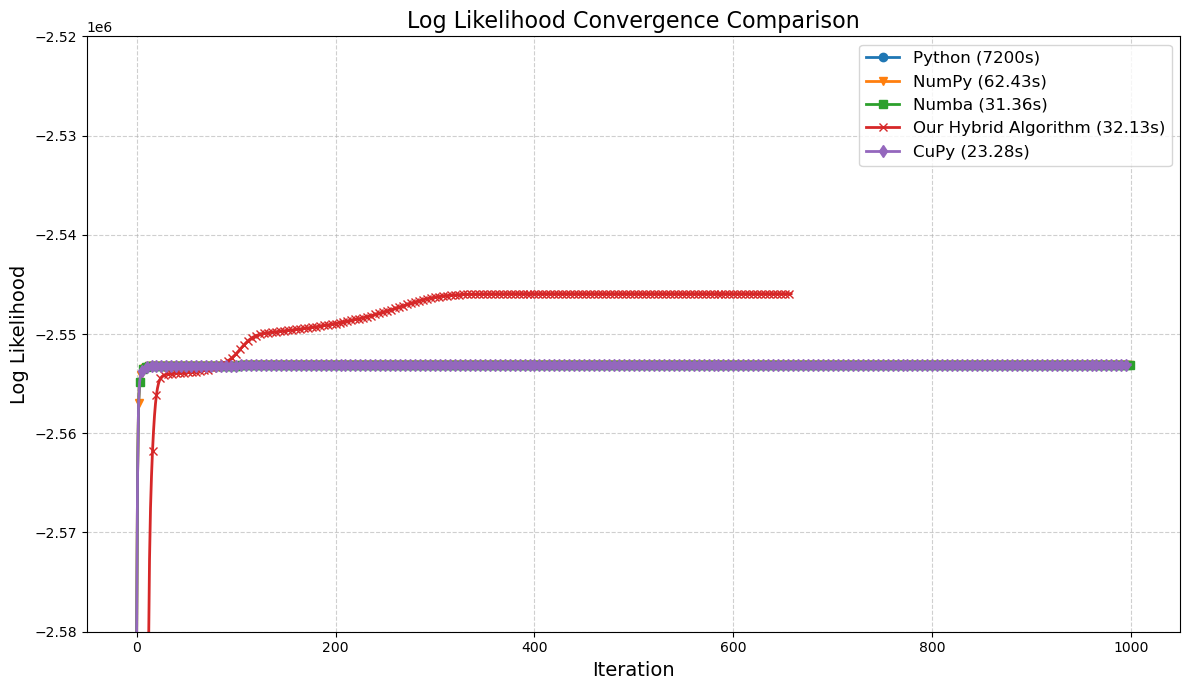
\includegraphics[width=0.35\textwidth]{azizi3.png}
    \caption{Convergence comparison with optimized Python libraries using different initialization strategies.}
\end{figure}

This experiment demonstrates that our implementation not only provides computational efficiency but also exhibits superior convergence properties, likely due to our enhanced numerical stability techniques. While the per-iteration time may be higher than highly optimized Python libraries for smaller datasets, our implementation requires fewer iterations to converge and handles larger datasets more effectively.

\subsection{Experiment 3: Testing our Hybrid Algorithm on IRIS Dataset}

To validate our hybrid algorithm on real-world data, we tested it on the classic Iris dataset, which contains 150 samples from three iris species with four features each (sepal length, sepal width, petal length, and petal width). The dataset presents an excellent benchmark for clustering algorithms due to its well-defined structure with one linearly separable class and two partially overlapping classes.

Our hybrid GMM implementation achieved excellent clustering results on this dataset, as evidenced by multiple evaluation metrics: Misclassification Rate (MCR) of 0.03333, Adjusted Rand Index (ARI) of 0.90387, and F-measure of 0.96658. These metrics indicate that our algorithm correctly identified the underlying clusters with high accuracy, making only 5 misclassifications out of 150 samples.

\begin{figure}[h!]
    \centering
    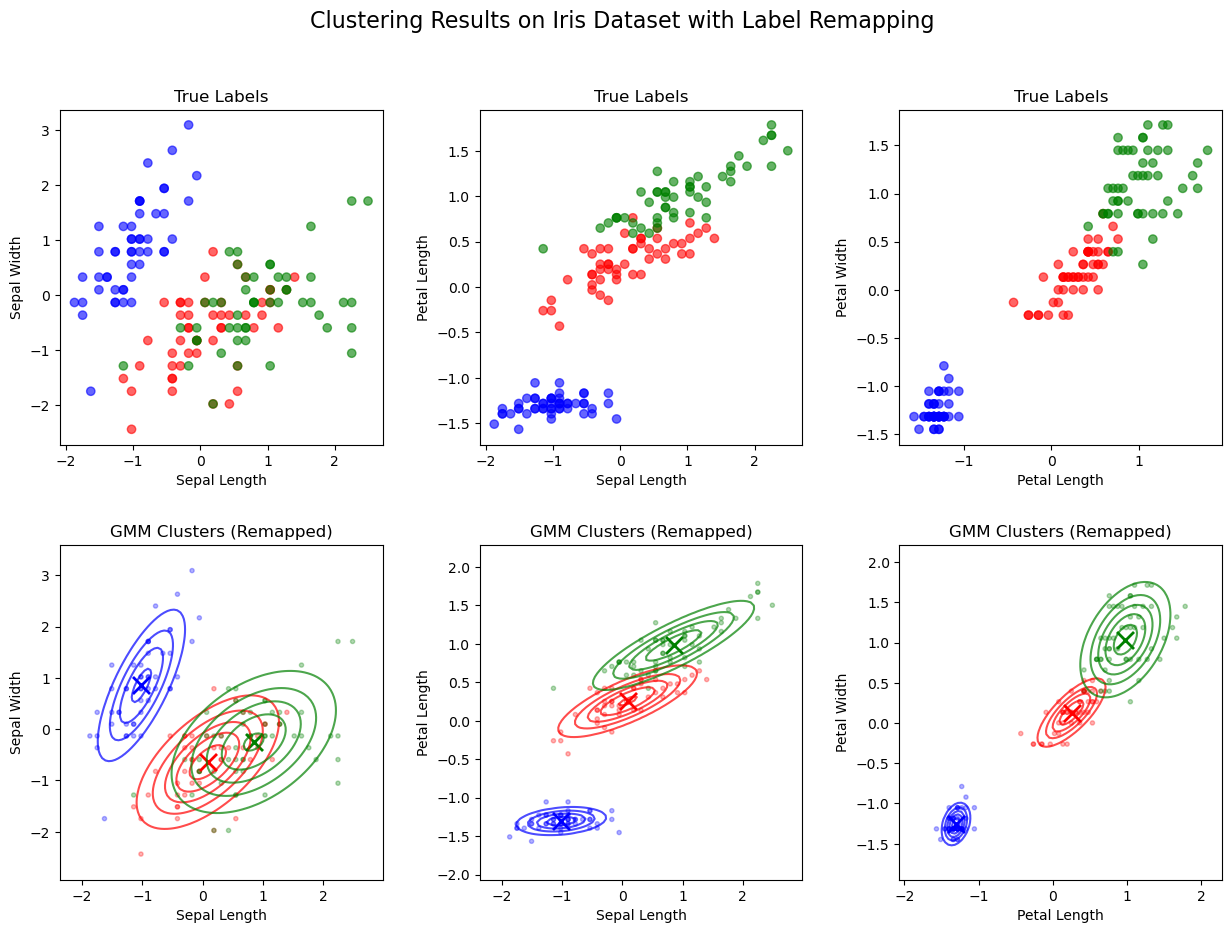
\includegraphics[width=0.35\textwidth]{iris1.png}
    \caption{Top row shows the true class labels across three feature pairs. Bottom row displays the fitted GMM clusters with corresponding density contours. The close match between true labels and model predictions demonstrates the algorithm's effectiveness at recovering the natural clusters in the data.}
    \label{fig:iris_results}
\end{figure}


\section{Conclusion and Future Work}
\label{conclusion}

In this paper, we presented a hybrid parallel implementation of the EM algorithm for GMMs that effectively leverages both GPU and CPU resources. The hybrid approach demonstrates very good performance compared to pure CPU and pure GPU implementations, with performance advantages that scale with dataset size and dimensionality. Details of the regularization techniques are not discussed here for brevity but can be found in our implementation.


Future work could explore several directions:
\begin{enumerate}
    \item \textbf{Optimized Linear Algebra Libraries}: Replacing Eigen with CUDA-optimized libraries like cuBLAS and cuSOLVER for matrix operations to further accelerate covariance computations and matrix inversions.
    
    \item \textbf{Sparse GMMs}: Implementing sparse covariance matrix representations for very high-dimensional data.
    
    \item \textbf{Integration with Deep Learning}: Exploring hybrid deep learning models that incorporate GMMs as components.
    
    \item \textbf{Distributed Implementation}: Extending our hybrid approach to distributed systems for handling extremely large datasets across multiple nodes.
    
    \item \textbf{Automatic Hyperparameter Tuning}: Developing mechanisms for automatically tuning regularization parameters and convergence criteria based on dataset characteristics.
\end{enumerate}

Our implementation demonstrates that effectively leveraging heterogeneous computing resources can significantly accelerate machine learning algorithms, enabling the analysis of larger and higher-dimensional datasets than previously practical.

\bibliographystyle{IEEEtran}
\begin{thebibliography}{11}

\bibitem{azizi2023parallel}
I.~Azizi, ``Parallelization in Python -- An Expectation-Maximization Application,'' Département des Opérations, Université de Lausanne, Jun. 2023. [Online]. Available: \url{https://iliaazizi.com/projects/em_parallelized/report.pdf}

\bibitem{kumar2009fast}
N.~S.~L. Phani Kumar, S. Satoor, and I. Buck, ``Fast parallel expectation maximization for Gaussian mixture models on GPUs using CUDA,'' in \emph{11th IEEE International Conference on High Performance Computing and Communications (HPCC)}, 2009, pp.~103--109. [Online]. Available: \url{https://ieeexplore.ieee.org/document/5166982}

\end{thebibliography}

\end{document}